\section{La persistenza}

Nel contesto di un sistema che prevede la gestione di eventi e impegni, è essenziale garantire che l’utente possa accedere in qualsiasi momento alla propria agenda, 
visualizzando gli appuntamenti più urgenti e pianificando efficacemente il proprio tempo. 
Deve perciò essere possibile trovare e mostrare nel minor tempo possibile i dati relativi all’agenda. 
Per soddisfare questo requisito, il recupero e la visualizzazione dei dati devono avvenire con la massima rapidità possibile, 
riducendo i tempi di latenza e ottimizzando il flusso di interazione con l’interfaccia utente. \\
\\
L’adozione di un meccanismo di salvataggio locale sui dispositivi offre il vantaggio di migliorare le prestazioni, 
consentendo un accesso immediato alle informazioni senza dover effettuare continue richieste al server remoto. 
Tuttavia, questa soluzione presenta dei limiti, in quanto non garantisce una persistenza a lungo termine dei dati né assicura la loro disponibilità su più dispositivi. 
Per superare tale criticità, è necessario definire una strategia di gestione della memoria che preveda una fonte di dati centrale e autorevole, 
alla quale tutti i dispositivi possano fare riferimento per recuperare e aggiornare le informazioni in modo coerente e affidabile.\\
\\
Un sistema di persistenza efficace deve quindi prevedere un meccanismo di sincronizzazione tra i dati salvati localmente e la loro controparte ufficiale memorizzata nel database centrale. 
Questo processo deve essere progettato in modo da garantire integrità, coerenza e scalabilità nelle interazioni, 
per essere resistente anche in presenza di un volume significativo di richieste concorrenti. 
La struttura del sistema di memorizzazione deve inoltre essere progettata tenendo conto del dominio applicativo e delle esigenze specifiche di utilizzo, 
al fine di assicurare un bilanciamento ottimale tra efficienza e robustezza operativa.\\
\\
Oltre alla gestione della persistenza dei dati per il singolo utente, è necessario affrontare il problema della condivisione e della modifica collaborativa delle informazioni. 
Poiché l’applicazione consente a più utenti di interagire sugli stessi eventi, le modifiche effettuate da un partecipante devono essere propagate in tempo reale agli altri dispositivi coinvolti. 
Questo introduce la necessità di implementare un sistema di aggiornamento distribuito, in grado di mantenere sincronizzati non solo i dispositivi di un singolo utente, 
ma anche quelli di tutti gli utenti interessati dalle modifiche.\\
\\
La gestione dell’accesso ai dati richiede quindi l’implementazione di un’architettura che preveda un punto di riferimento centrale chiaro e affidabile, 
capace di fungere da fonte primaria delle informazioni. 
Al tempo stesso, l’utilizzo di copie locali dei dati sui dispositivi client consente di ridurre l’impatto delle latenze di rete, 
migliorando la reattività dell’interfaccia e offrendo un’esperienza utente più fluida.\\
\\
L’adozione di una memoria centrale unica garantisce l’integrità e l’affidabilità dei dati ufficiali, 
fornendo un punto di accesso sicuro per la consultazione e la modifica delle informazioni. 
Tuttavia, questa scelta introduce la necessità di gestire due livelli distinti di responsabilità: 
da un lato, il client deve occuparsi di mantenere aggiornati i dati memorizzati localmente, 
mentre il server deve garantire la corretta distribuzione delle modifiche agli altri dispositivi interessati. 
La sincronizzazione e la gestione delle versioni dei dati diventano quindi elementi chiave per assicurare la coerenza del sistema e prevenire eventuali conflitti tra modifiche concorrenti.

\clearpage
\subsection{Memoria principale}

	

Nell’implementazione di applicazioni scalabili, la gestione del salvataggio dei dati può essere strutturata secondo un modello centralizzato o distribuito, 
a seconda delle esigenze di affidabilità, scalabilità e prestazioni del sistema. 
L’adozione di un’architettura di memoria distribuita offre molteplici vantaggi, tra cui una maggiore resilienza ai guasti di una singola fonte, 
la riduzione del carico di memoria su un'unica risorsa di archiviazione e una migliore scalabilità complessiva del sistema. 
Tuttavia, questa soluzione introduce una maggiore complessità infrastrutturale, poiché richiede meccanismi avanzati per garantire la persistenza, 
l’affidabilità e la consistenza delle informazioni.\\
\\
Salvo specifici requisiti che rendano indispensabile la distribuzione totale o parziale della memoria, 
una strategia basata su un database centralizzato può risultare più efficiente dal punto di vista prestazionale e semplificare la gestione complessiva del sistema. 
L’adozione di un’architettura centralizzata consente infatti di ottimizzare i tempi di accesso ai dati e ridurre la latenza delle operazioni, 
a fronte di una minore complessità nella sincronizzazione e nel mantenimento della consistenza delle informazioni.\\
\\
\subsubsection{I database e la scalabilità}

I database si suddividono in due macro categorie principali: relazionali e non relazionali. 
I database relazionali si caratterizzano per strutture dati rigide e schematizzate, che consentono di stabilire connessioni tra le diverse risorse in tempi estremamente rapidi. 
Viceversa, i database non relazionali offrono una maggiore flessibilità strutturale, permettendo l’archiviazione di dati eterogenei con un accoppiamento più debole tra le entità. 
Questa caratteristica li rende particolarmente adatti a scenari in cui è richiesta un'elevata scalabilità orizzontale e in cui il volume di richieste è significativo.\\
\\

La scelta della tipologia di database più appropriata dipende strettamente dalle esigenze specifiche del progetto. 
I database relazionali sono gli unici in grado di garantire le proprietà di Atomicità, Consistenza, Isolamento e Durabilità (ACID), 
grazie all’implementazione di un rigoroso sistema di transazioni. 
Questo meccanismo, se da un lato assicura un’elevata affidabilità dei dati, dall’altro introduce un temporaneo blocco delle risorse durante le operazioni di scrittura, 
potenzialmente influenzando le prestazioni complessive del sistema.\\
\\
Dal punto di vista della scalabilità, invece, i principali fattori da considerare includono il rapporto tra operazioni di lettura e scrittura, 
la natura dei dati gestiti e la relazione tra le entità. 
Le operazioni di lettura possono essere ottimizzate tramite la creazione di copie dei dati e la parallelizzazione dei processi, 
permettendo di soddisfare un elevato numero di richieste simultanee.\\
\\

Al contrario, le operazioni di scrittura possono introdurre ritardi significativi, in quanto implicano la temporanea indisponibilità della risorsa fino al completamento dell’aggiornamento. 
In alcuni casi, in base alla tipologia del database, ciò può invalidare le copie presenti nel sistema fino alla propagazione dell’aggiornamento, 
compromettendo temporaneamente la consistenza delle informazioni. 
Grazie alla loro struttura flessibile e a requisiti meno stringenti in termini di garanzia ACID, 
i database non relazionali risultano generalmente più efficienti in contesti caratterizzati da operazioni di scrittura frequenti.\\
\\

Quando il sistema richiede una gestione dinamica delle informazioni, con dati opzionali o variabili, i database non relazionali offrono un livello di adattabilità superiore. 
Il salvataggio delle informazioni in forma di documenti consente infatti di modificare la struttura dei dati senza la necessità di riconfigurare lo schema del database, 
garantendo una maggiore elasticità. Tuttavia, questa necessità si manifesta prevalentemente in casi specifici, che rappresentano solo una parte del dominio applicativo complessivo. \\
\\

\subsubsection{La gestione delle relazioni tra le entità}
Un aspetto critico nella scelta del database riguarda la gestione delle relazioni tra le entità. 
È fondamentale analizzare la distribuzione delle richieste per ciascun elemento e il carico computazionale associato a ogni operazione. 
Tra le operazioni più costose in termini di prestazioni, che più ostacola e rallenta il recupero dei dati, vi è l’operazione di unione necessaria. 
Durante le operazioni di unione vengono incrociati i dati di vari elementi per restituire un oggetto coerente che presenti tutte le proprietà necessarie, 
originariamente distribuite in molteplici tabelle. 
L’esecuzione di unione su database relazionali, pur essendo ottimizzata, 
introduce azioni computazionali di grande entità che possono impattare significativamente sui tempi di risposta delle richieste. 
Per questo motivo si cerca di ridurre il più possibile le richieste che comportano l’incrocio di dati da tabelle diverse. \\
\\
Le relazioni tra elementi possono essere classificate in tre categorie principali: 
di tipo uno a uno, uno a molti, e molti a molti. \\
Nelle relazioni uno a uno il recupero dei dati è diretto e richiede uno sforzo computazionale limitato. 
Nei casi uno a molti e molti a molti il reperimento delle informazioni richiede un’attenta valutazione delle modalità di accesso per ottimizzare le prestazioni: 
in questo caso, una delle strategie possibili per migliorare l’efficienza delle richieste offerte dai database non relazionali è il salvataggio per copia del dato all’interno dell’oggetto. 
Questa operazione risulta efficiente se le richieste sono sproporzionate verso una delle due parti.\\
\\
Ad esempio, in una relazione uno a molti, nel caso in cui la richiesta di quell’elemento non sia frequente ma sia importante ottenere gli elementi collegati; 
conviene copiare gli oggetti relativi all’interno dell’elemento singolo. 
L’impostazione inversa, in cui si copia il singolo all’interno dei molti elementi, 
comporterebbe l’ispezione di tutti i componenti esistenti alla ricerca di quelli che contengono l’elemento dato. 
Se però, viceversa, sono frequenti le richieste relative agli elementi multipli, e la loro relazione è importante, 
conviene copiare il singolo all'interno di detti elementi, per evitarne il recupero ogni volta.\\
\\
I database relazionali non permettono la copia di elementi all’interno di altri, ma sono ottimizzati per unire tra loro tabelle, 
richiedendo comunque tempistiche e capacità elaborative non indifferenti. \\
\\
Tuttavia, non vi è alcun vincolo che impedisca l’affiancamento di database di tipologia diversa per rispondere a esigenze specifiche e sfruttare i punti di forza di entrambe le tecnologie.

\subsubsection{Analisi del dominio}

La scelta del database deriva da un’attenta analisi delle principali interazioni tra gli elementi del dominio. 
Il dominio descrive i componenti dell’applicazione e le loro relazioni. 
In particolare, vengono espresse le dipendenze, i rapporti reciproci e le cardinalità delle relazioni. 
A titolo esemplificativo, dal diagramma del dominio si deduce che ad un oggetto Event possono corrispondere più oggetti Photo, 
ma soprattutto che l’oggetto Photo è strettamente legato all’oggetto Event.\\
\\
\begin{figure}[h!]
    \centering
    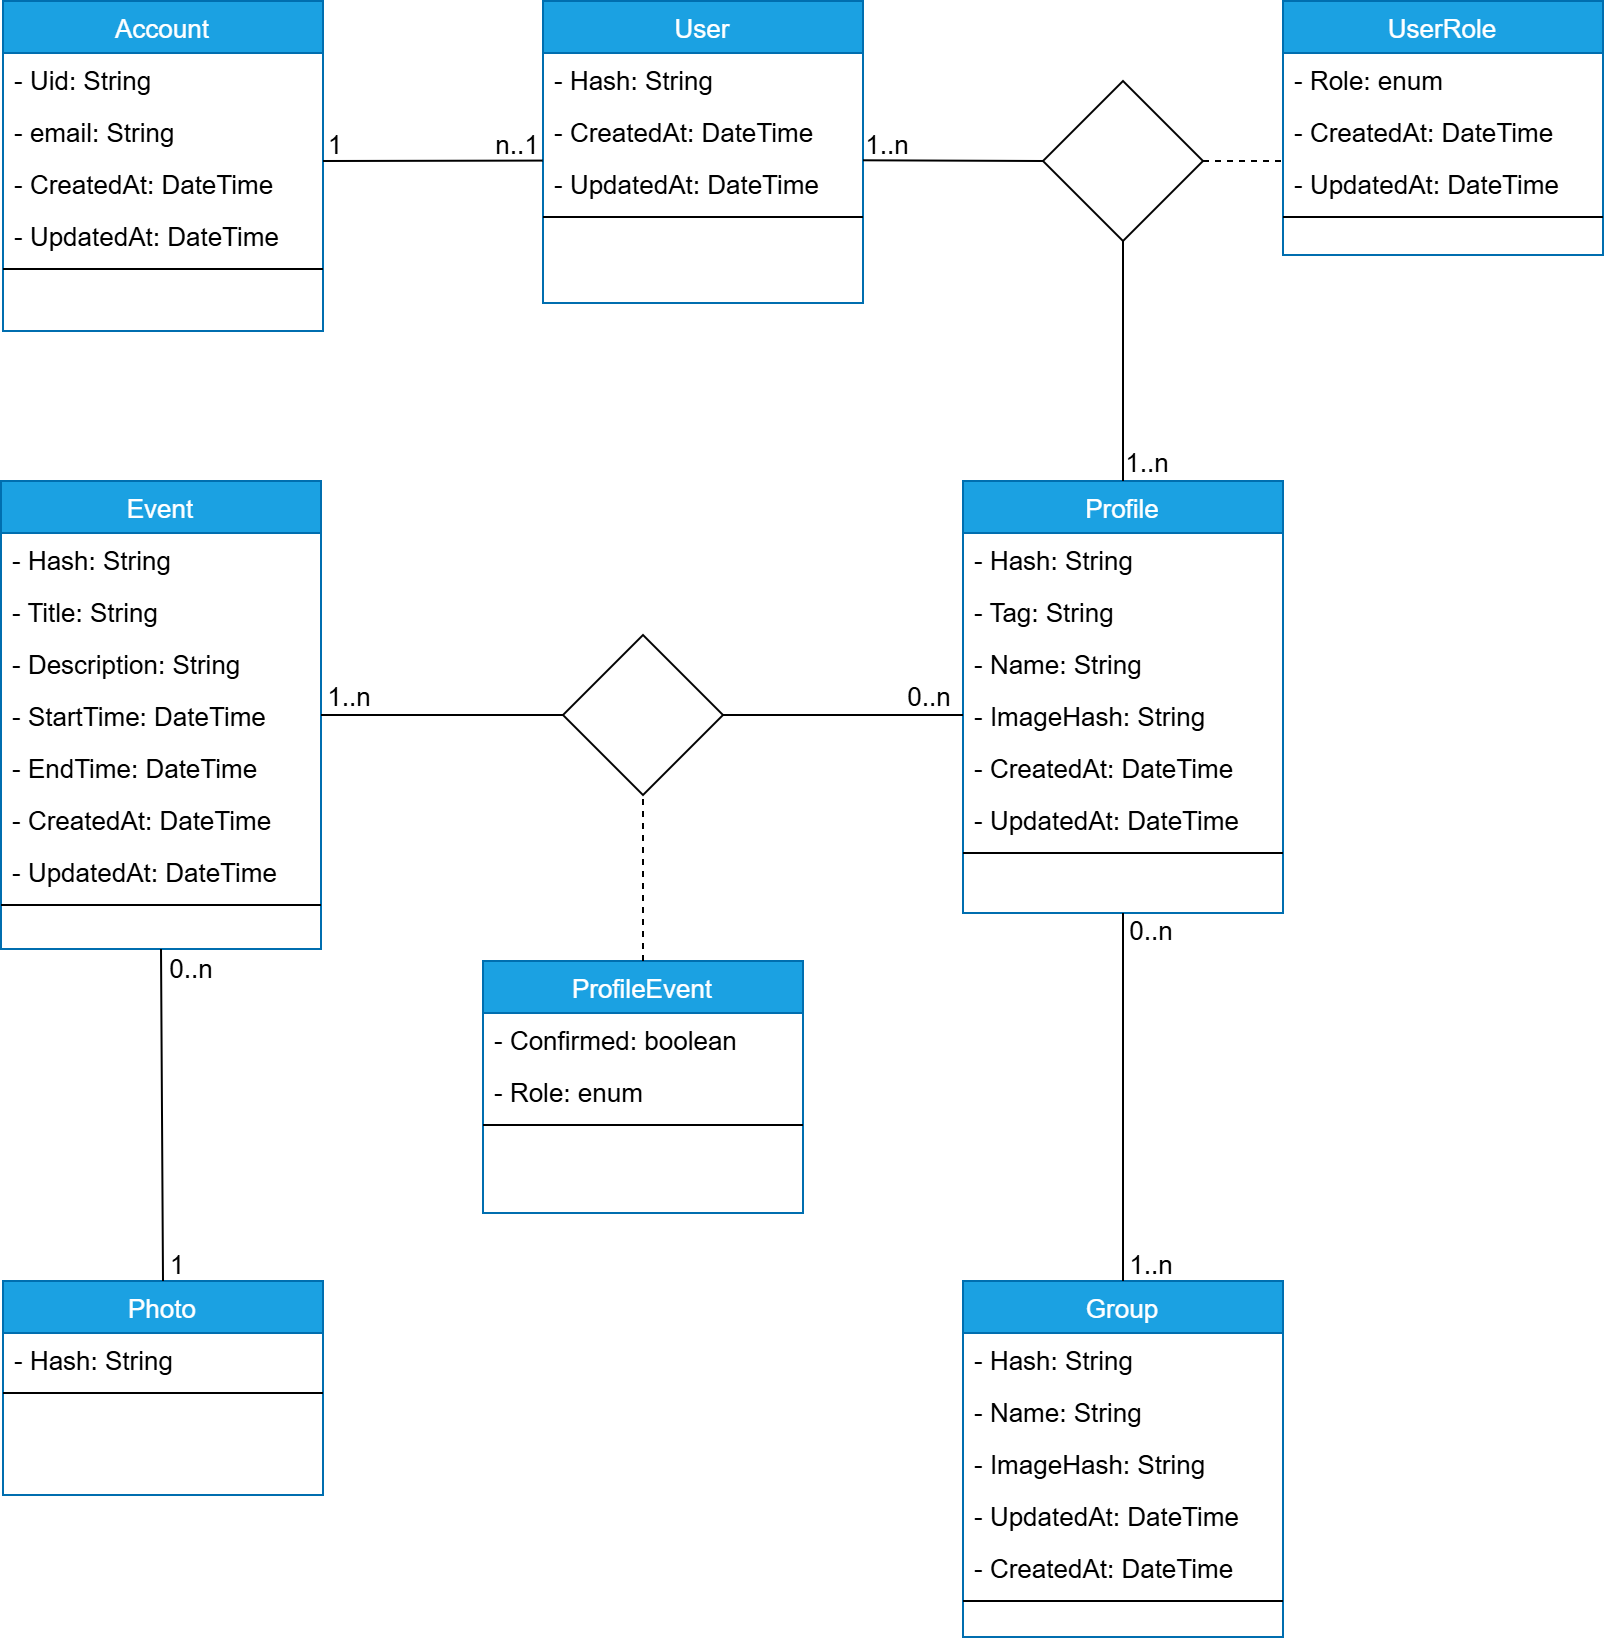
\includegraphics[width=\textwidth]{ProgettoDominioServer.png}
    \caption{Diagramma del dominio}
\end{figure}
Le richieste riguardo alle informazioni tra Account, User e Profile, con i relativi UserRole, vengono eseguite all’avvio del programma, per poi essere mantenute in memoria locale. 
Le modifiche a questi elementi sono sporadiche.
Allo stesso modo gli oggetti Group vengono recuperati solo all’avvio dell’applicazione, e, salvo rari aggiornamenti, non occupano ulteriormente lo spazio delle richieste.\\
\\
La maggioranza delle richieste verterà sull’ottenimento dei dati relativi agli Event e ai Profile. 
Infatti ad ogni avvio dell’applicazione sarà richiesto di recuperare gli eventi di ogni profilo, mentre, ogni volta che si apre il dettaglio di un evento, 
sarà necessario recuperare i rispettivi dati, includendo i profili associati. 
Si prevede che la cardinalità dei profili associati ad un evento risieda nell’ordine delle decine, 
mentre agli eventi che si associano ai profili l’ordine di grandezza previsto risiede nelle migliaia. \\
\\

La relazione che accomuna Event e Profile è di tipologia molti a molti, identificata con l’oggetto ProfileEvent. 
L’elemento ProfileEvent, oltre a descrivere la relazione, contiene la proprietà Confirmed, che indica la conferma di partecipazione di un profilo ad un evento. 
Vista la natura del progetto, la proprietà Confirmed, assieme ai dati degli Event, sarà tra i campi che subiranno modifiche con maggiore frequenza.\\
\\
Riassumendo, le operazioni principali che vertono sulle prestazioni del database sono il recupero degli eventi relativi ai profili, il recupero dei profili collegati agli eventi, 
l’aggiornamento dei campi degli oggetti Event e la modifica del campo Confirmed relativa ai ProfileEvent.\\
\\

Nonostante sia più probabile che venga richiesto il dettaglio di un evento, e quindi sia più frequente il dover recuperare i Profile relativi all’Event, 
la proporzione delle richieste prevista non giustifica lo sbilanciamento della relazione sugli Event.
Infatti, se si salvassero tutti i ProfileEvent sull’oggetto Event, le richieste degli eventi appartenenti ai profili, sebbene meno frequenti, 
richiederebbero l’ispezione di tutti gli Event alla ricerca del Profile indicato. 
Infine, se si duplicasse l’oggetto ProfileEvent, oltre che nella sua tabella originaria, anche sugli Event la sua creazione, 
la sua eliminazione e la modifica del campo Confirmed richiederebbero il doppio delle scritture.\\
\\
Vista quindi la necessità di letture frequenti da entrambe le parti di una relazione molti a molti e la necessità di scrittura dell’oggetto che la identifica, 
si individua in un database relazionale la soluzione più efficace per il dominio del progetto. 
Infatti, i database relazionali sono ottimizzati sulle operazioni di unione tra tabelle, garantendo velocità di recupero in lettura da entrambe le parti. 
Permettendo la separazione delle tabelle e gestendo gli oggetti ProfileEvent come entità indipendenti, 
la modifica del campo Confirmed comporta il blocco del solo elemento ProfileEvent. 
Le caratteristiche ACID forniscono inoltre uno stato centrale per tutta l’applicazione, che, 
per quanto non strettamente necessario, garantisce l’uniformità delle informazioni per tutti gli utenti.\\
\\

\clearpage
\subsubsection{La scelta del database}

Azure offre un’ampia scelta di database relazionali che possono essere integrati con il resto dell’ecosistema. 
Oltre alla tecnologia proposta, nella scelta del database più adatto bisogna considerare soprattutto l’integrazione con servizi accessori, 
le particolarità del server su cui viene eseguito, e i costi che si andrà ad affrontare.\\
\\
\begin{figure}[h!]
    \centering
    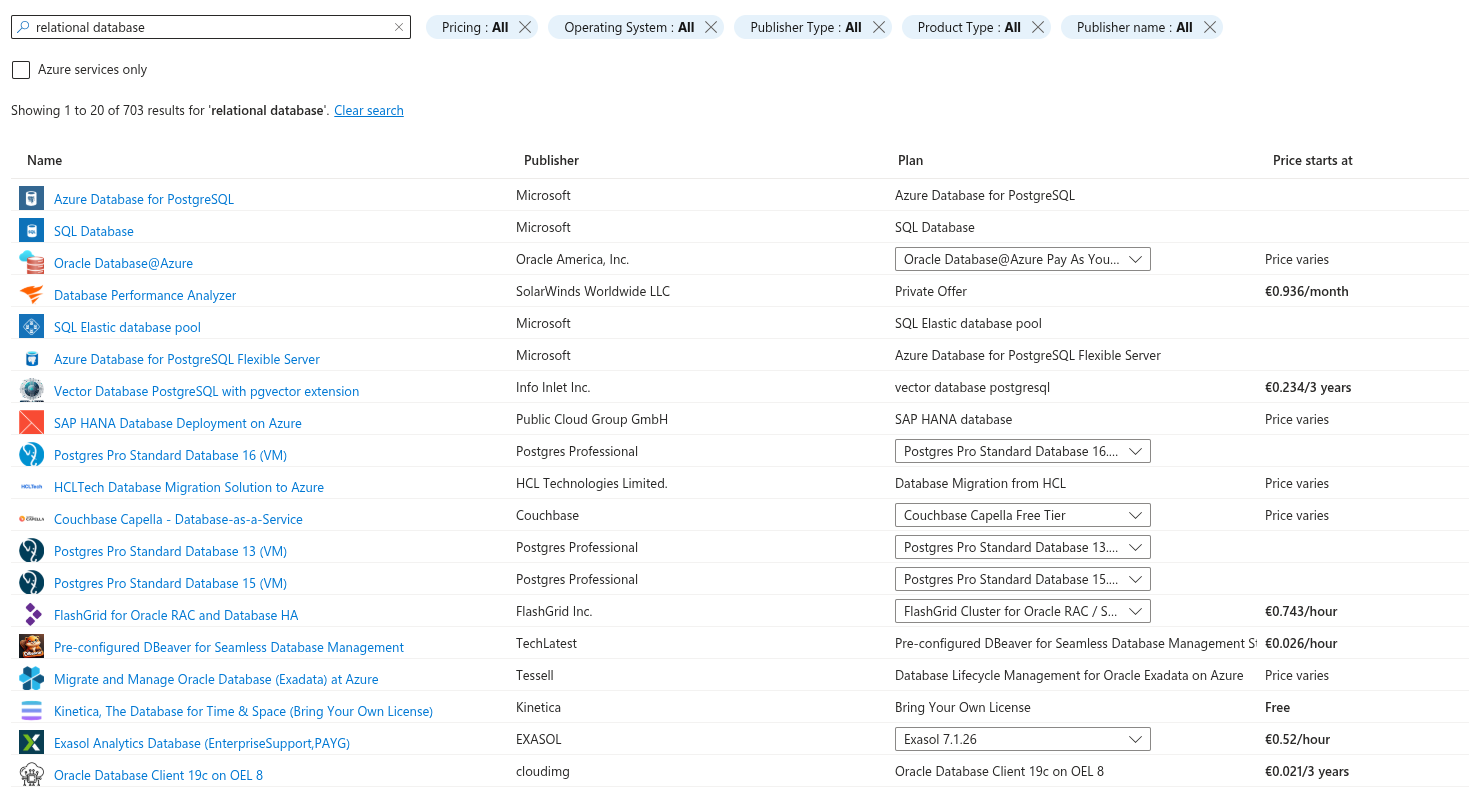
\includegraphics[width=\textwidth]{Possibilitadelcloud.png}
    \caption{Proposte di Azure per i database relazionali}
\end{figure}	


A meno di necessità particolari che richiedono l’utilizzo di una tecnologia implementata da uno specifico database, 
la grande sovrapposizione di funzionalità delle diverse offerte di database relazionali presenti sul mercato garantisce 
il  soddisfacimento delle necessità rilevate dall’analisi del dominio indipendentemente dalla tecnologia proposta dal servizio.\\
\\
La grande differenza tra i vari servizi sta nelle proprietà del server incaricato di fornire il potere computazionale necessario per l’esecuzione. 
L’architettura del server e la sua integrazione con la tecnologia del database, infatti, determinano l’effettiva capacità di scalabilità del servizio.\\
\\
Si intende scalabilità verticale la capacità di aumentare le risorse della stessa macchina in cui si esegue il codice. 
La scalabilità verticale viene definita nel momento di creazione del servizio, in cui si determinano le risorse da dedicare alla macchina che esegue il programma. 
Trattandosi di macchine virtualizzate, è sempre possibile in un secondo momento aumentare le prestazioni in caso di necessità.\\
\\

Per scalabilità orizzontale si intende invece la capacità di delegare il carico di lavoro ad altre macchine, eventualmente coordinando le modifiche. 
Questo permette una risposta alle richieste più resistente, riducendo il rischio di colli di bottiglia che potrebbero venirsi a formare nell’utilizzo di un nodo singolo.
La scalabilità orizzontale richiede però l’implementazione di tecnologie apposite integrate con il database che permettano l’esecuzione in nodi fisici differenti. \\
\\
Una volta individuata la tecnologia adatta e il livello di scalabilità desiderati, 
è bene considerare le altre necessità o le opportunità aggiuntive generate dalla presenza di un database nel progetto. \\
\\

L’alta disponibilità(HA) è la proprietà di garantire l’accesso al servizio nonostante i guasti. 
Ad esempio, si può mantenere una macchina identica al server principale in grado di replicare il servizio, spostando il carico in caso di guasto del server principale. 
Si misura in “numero di nove”, ovvero la quantità di nove presenti nella percentuale del tempo per il quale si garantisce la disponibilità del servizio.
I servizi offrono diverse qualità di HA, in base alle funzionalità desiderate.\\
\\

Alcuni servizi possono presentare offerte di backup per riportare il server nello stesso stato di qualche momento precedente. 
Questo permette il ripristino del sistema ad un punto precedente rispetto all’avvenimento di eventuali errori o guasti del sistema.\\
\\

Inoltre, Azure mette a disposizione molteplici servizi accessori che possono essere uniti al servizio. 
Questo permette di estendere le potenzialità del database tramite  l’analisi e il monitoraggio dei dati, 
generando prestazioni aggiuntive o integrando i dati per lo sviluppo di altre tecnologie.\\
\\
Infine è necessario controllare i costi che le scelte progettuali e prestazionali hanno comportato: 
pur generalmente legati al consumo effettivo delle risorse, e quindi in grado di fornire solo una previsione del costo finale, 
ogni decisione presa conduce ad un possibile aumento di prezzo, 
ed è quindi bene controllare che le risorse selezionate siano effettivamente  necessarie a soddisfare i requisiti del progetto.\\
\\
Riducendo al minimo i costi, visto l’utilizzo iniziale dell’applicazione, e nessuna necessità tecnologica specifica, 
la scelta del database per la persistenza del progetto è ricaduta su Azure SQL Database. 
Presentando un database relazionale di tecnologia proprietaria di Microsoft, Azure SQL database esegue su un solo nodo, 
fornendo però la possibilità di  scalare  verticalmente tramite la possibilità di modificare le risorse assegnate in ogni momento, 
garantendo comunque prestazioni soddisfacenti per il servizio.\\
\\
Al server principale è stata affiancata una replica che rimane costantemente aggiornata. 
Situata in una località differente dal server principale, garantisce alta disponibilità continuando a fornire i servizi anche in caso di malfunzionamenti al server principale.
\clearpage
\subsubsection{Le limitazioni dei database relazionali}

La scelta di un database relazionale può però comportare limitazioni a livello prestazionale. 
Il più grande tallone d'Achille dei database relazionali è il numero limitato di connessioni contemporanee permesso. 
Questo comporta un numero massimo di richieste in contemporanea che il database può gestire, minacciando la scalabilità. \\
\\

Per ovviare ai problemi di scalabilità ci sono diverse soluzioni non esclusive che possono migliorare le prestazioni. 
Sicuramente si deve limitare al minimo il tempo in cui ogni richiesta mantiene la connessione, 
distinguendo nel codice momenti precisi e definiti in cui vengono richieste le modifiche al database. \\
\\  

Inoltre, si può interporre un livello di caching tra la logica applicativa e le richieste al database. 
Il livello di caching si occupa di gestire le richieste al database fornendo e duplicando le risposte che possiede già in memoria, 
eventualmente centralizzando le richieste in caso i dati siano invece da recuperare. 
Per i dati in scrittura, invece, salva temporaneamente le modifiche richieste, aggiornando subito la memoria locale, 
per poi apportare le modifiche al database in momenti di carico ridotto. 
Garantisce così un tempo di risposta e di propagazione degli aggiornamenti ridotto. 
Questo consente di alleviare le richieste al database, estendendo di molto le prestazioni fornite.\\
\\

Nel caso in cui però fossero necessarie ulteriori prestazioni, se il dominio e i requisiti lo permettono, 
si può eventualmente delegare ad un database non relazionale le modifiche ai dati e alle relazioni che non necessitano delle qualità ACID ma richiedono un’alta frequenza di scrittura.\\
\\ 
Infine, se fosse necessario mantenere un database relazionale, 
per aumentare le prestazioni conviene cambiare architettura e adottarne una che supporti la scalabilità orizzontale, per suddividere il carico su più nodi.
\clearpage


\subsubsection{L' integrazione con C\#}

La scelta di un database relazionale per la persistenza ha comportato sviluppi progettuali precisi. 
In primis si rende necessario tradurre il dominio in componenti relazionali che possano essere espressi e salvati nelle tabelle del database.

\begin{figure}[h!]
    \centering
    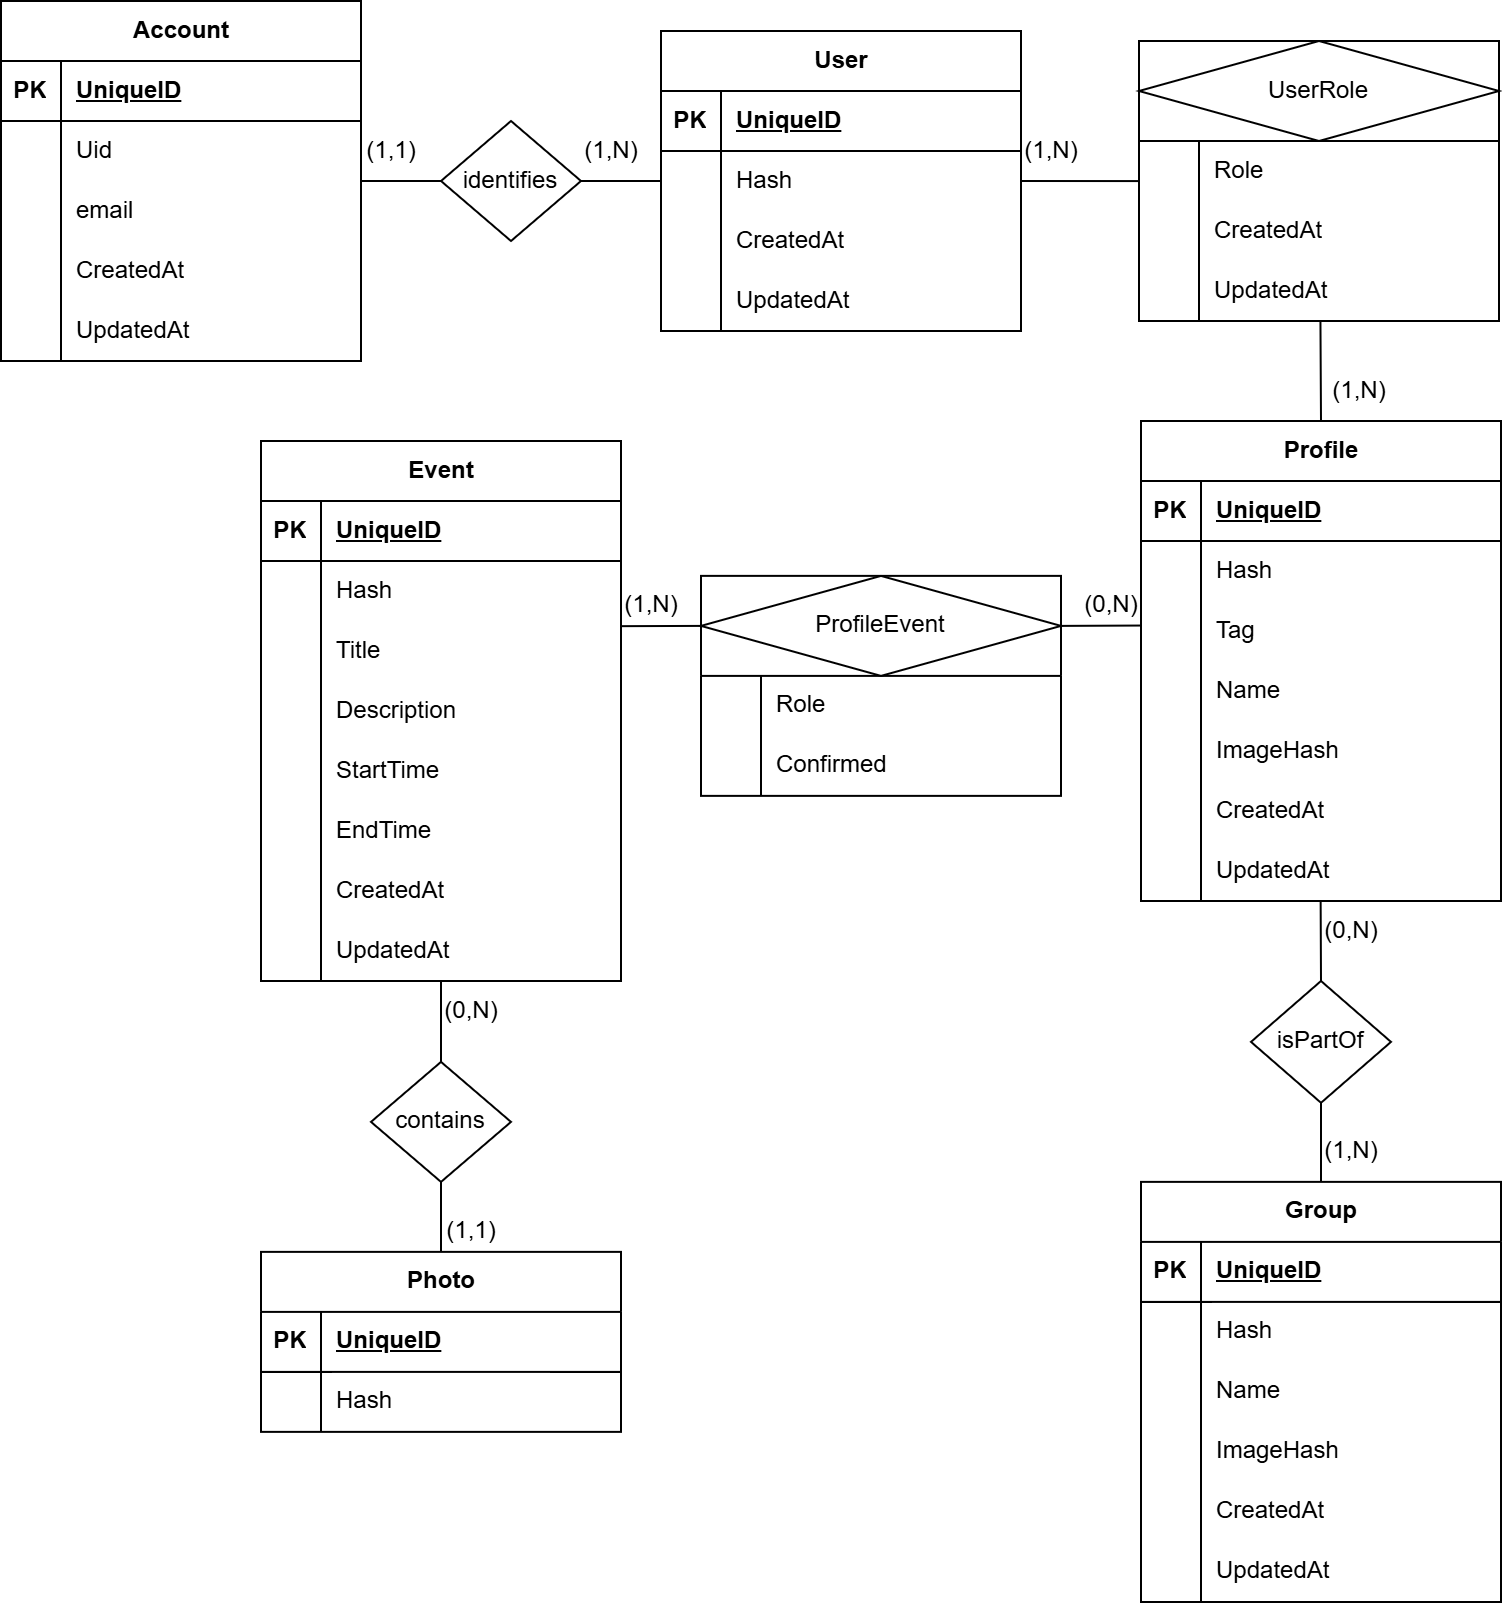
\includegraphics[width=\textwidth]{ProgettoDiagrammaER.png}
    \caption{Diagramma Entità - Relzione del dominio}
\end{figure}	

Si creano quindi sul server le classi logiche del programma, a partire dal dominio. 
Ogni classe corrisponde ad un oggetto del dominio, presentando i valori e le relazioni dei componenti come attributi dell’oggetto.\\
\\
Entity Framework Core di .Net(EFCore) è una libreria di C\# che permette di unire le classi logiche del programma alle tabelle del database. 
Fornisce un’astrazione logica del collegamento con il database e le richieste relative, fornendo una rappresentazione di alto livello delle connessioni sottostanti. \\
\\
Una volta collegato il server con il database tramite le stringhe di connessione salvate sull’Azure Key Vault, 
sono state definite le proprietà tra le varie entità, per poi inizializzare in automatico la struttura del database. 
Le modifiche alla struttura del database vengono infatti generate automaticamente da EFCore in seguito alla creazione o alla modifica degli attributi degli oggetti. 
Questo permette di star dietro agli aggiornamenti, generando e salvando le modifiche da applicare ad ogni modifica delle proprietà del dominio.\\
\\
\begin{figure}[h!]
    \begin{center}
        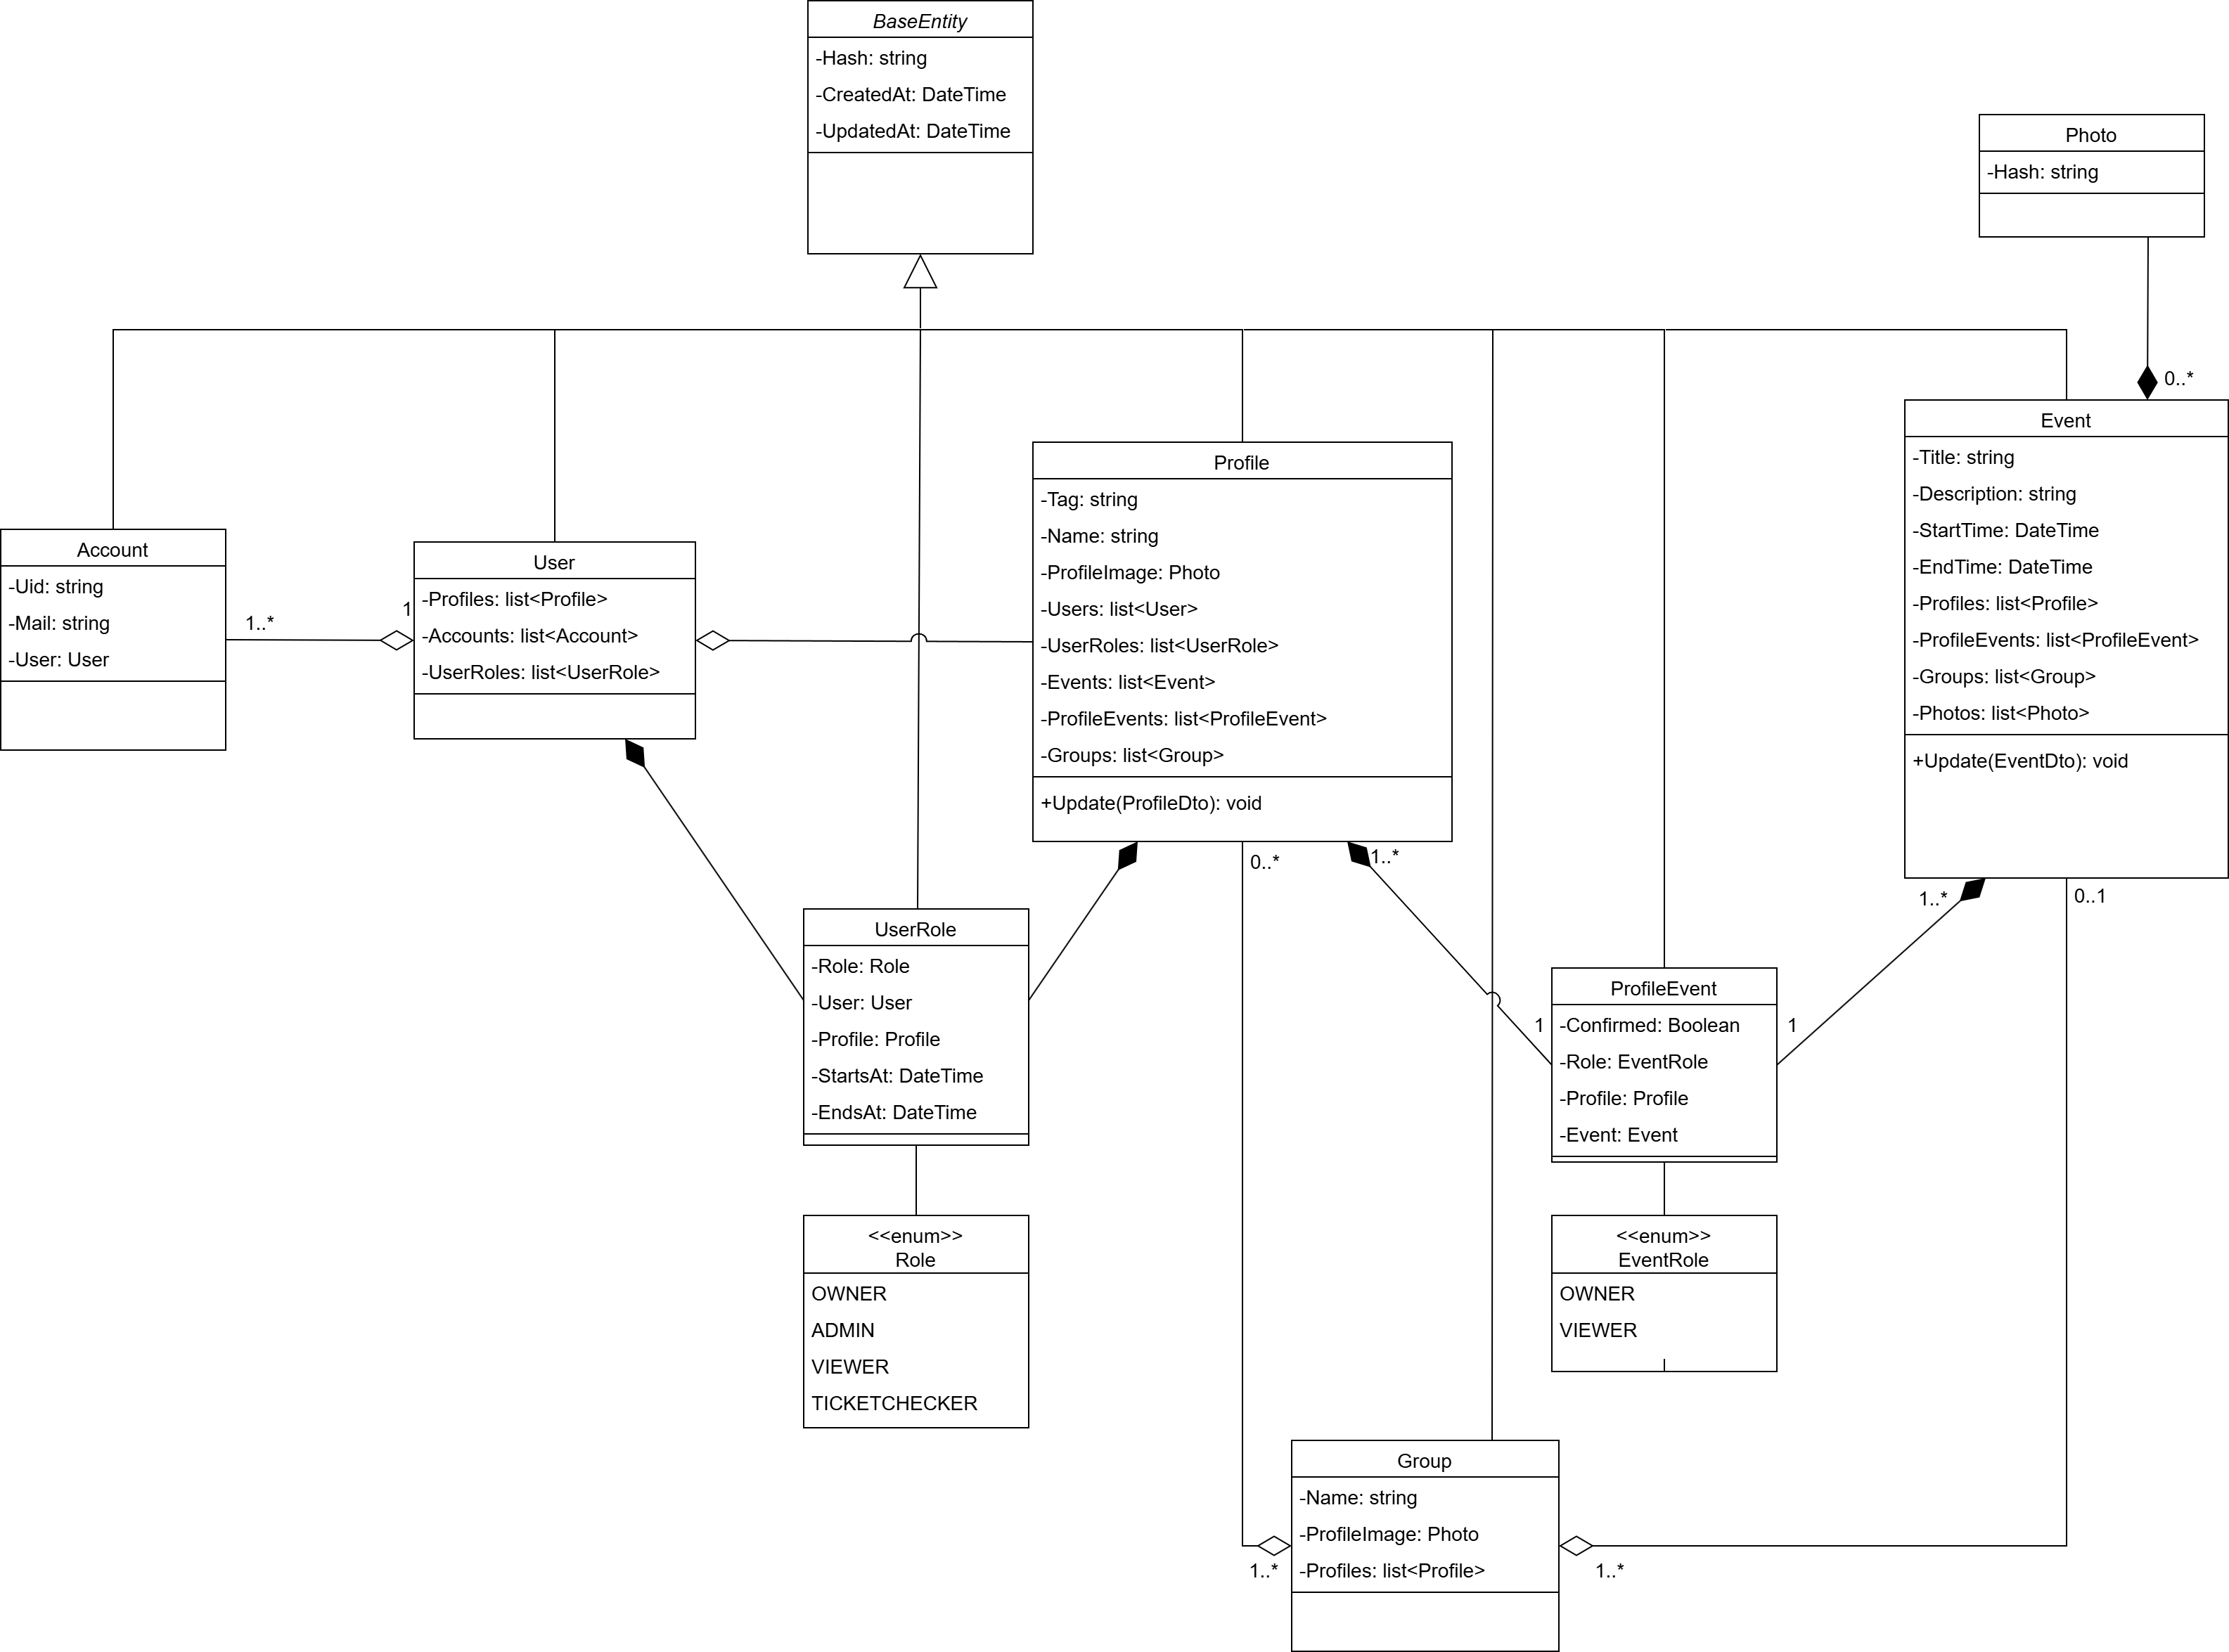
\includegraphics[width=\textwidth]{ModelClassDiagram.png}
        \caption{Modello delle classi del client}
    \end{center}
\end{figure}

Per la riduzione del carico computazionale richiesto da elementi con tante relazioni si utilizza la tecnica del lazy loading. 
La tecnica del Lazy Loading consiste nel richiedere i dati delle relazioni di un elemento solo quando strettamente necessario. 
La sua realizzazione tramite EFCore è attuata grazie alla proprietà virtual, 
che permette di gestire un oggetto con un riferimento al database richiedendo i dati delle sue relazioni solo quando viene espressamente richiesto.
\clearpage
\subsection{Cache Locale}

Richiedere e ottenere dati dal server comporta ritardi che impattano sulle prestazioni. 
Se la tecnologia del dispositivo lo permette, è utile salvare copie delle informazioni usate più frequentemente nella memoria locale del dispositivo. 
Nel momento di una interazione che richiede la ricerca dei dati, si possono fornire le informazioni disponibili in copia, 
per poi eventualmente aggiornarle se si rivelassero imprecise. Questo permette un tempo di risposta apparente minore e una migliore esperienza utente.\\
\\
\subsubsection{Creazione della memoria locale}
Non tutti i dispositivi permettono una gestione della memoria a lungo termine. 
In particolare, i browser web non presentano questa funzionalità, ma i dispositivi mobili e i programmi sì. \\
\\
Per motivi di prestazioni, il framework Flutter nativamente mantiene lo stato di un componente solo il tempo strettamente necessario per la sua esecuzione. 
Il tempo di vita dello stato coincide normalmente con quello del componente a cui è associato. 
La normale persistenza degli elementi e dei dati ha durata limitata. 
Si rende necessaria la creazione e la gestione di una cache locale che permetta di mantenere i dati ricevuti dal server anche in seguito al termine di servizio dei componenti.\\
\\
\begin{figure}[h!]
    \centering
    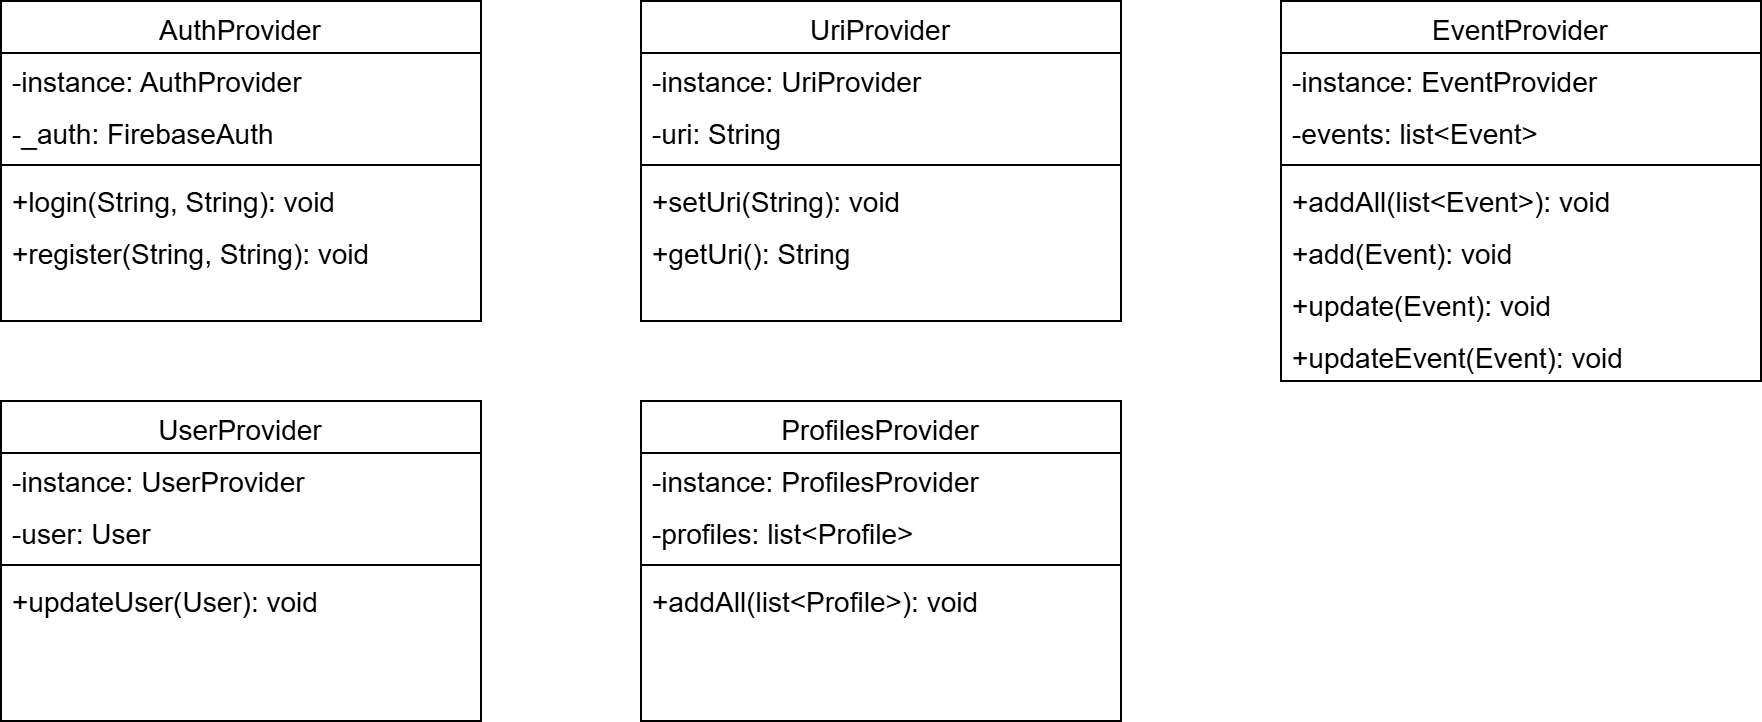
\includegraphics[width=\textwidth]{FrontProviderClassDiagram.png}
    \caption{Classi provider all'interno dell'applicazione}
\end{figure}	
La cache locale viene suddivisa in base alle classi logiche del dominio, ed è accessibile tramite servizi dedicati. 
In particolare, grazie a componenti di tipologia provider è possibile aggiornare in automatico le parti dell’applicazione interessate dalle modifiche. 
Al termine di una richiesta dati al server, il provider viene notificato, salvando il dato in memoria e scatenando un aggiornamento a catena sui componenti interessati.\\
\\
La cache deve essere unica e disponibile in tutto il programma. 
I provider attraverso cui si realizza la cache locale seguiranno il pattern singleton, che garantisce l’unicità dell’elemento all’interno del programma. 
Una volta creati all’avvio del programma, infatti, tutti gli elementi dell’applicazione avranno accesso agli stessi dati, quando necessario.

\begin{figure}[h!]
    \centering
    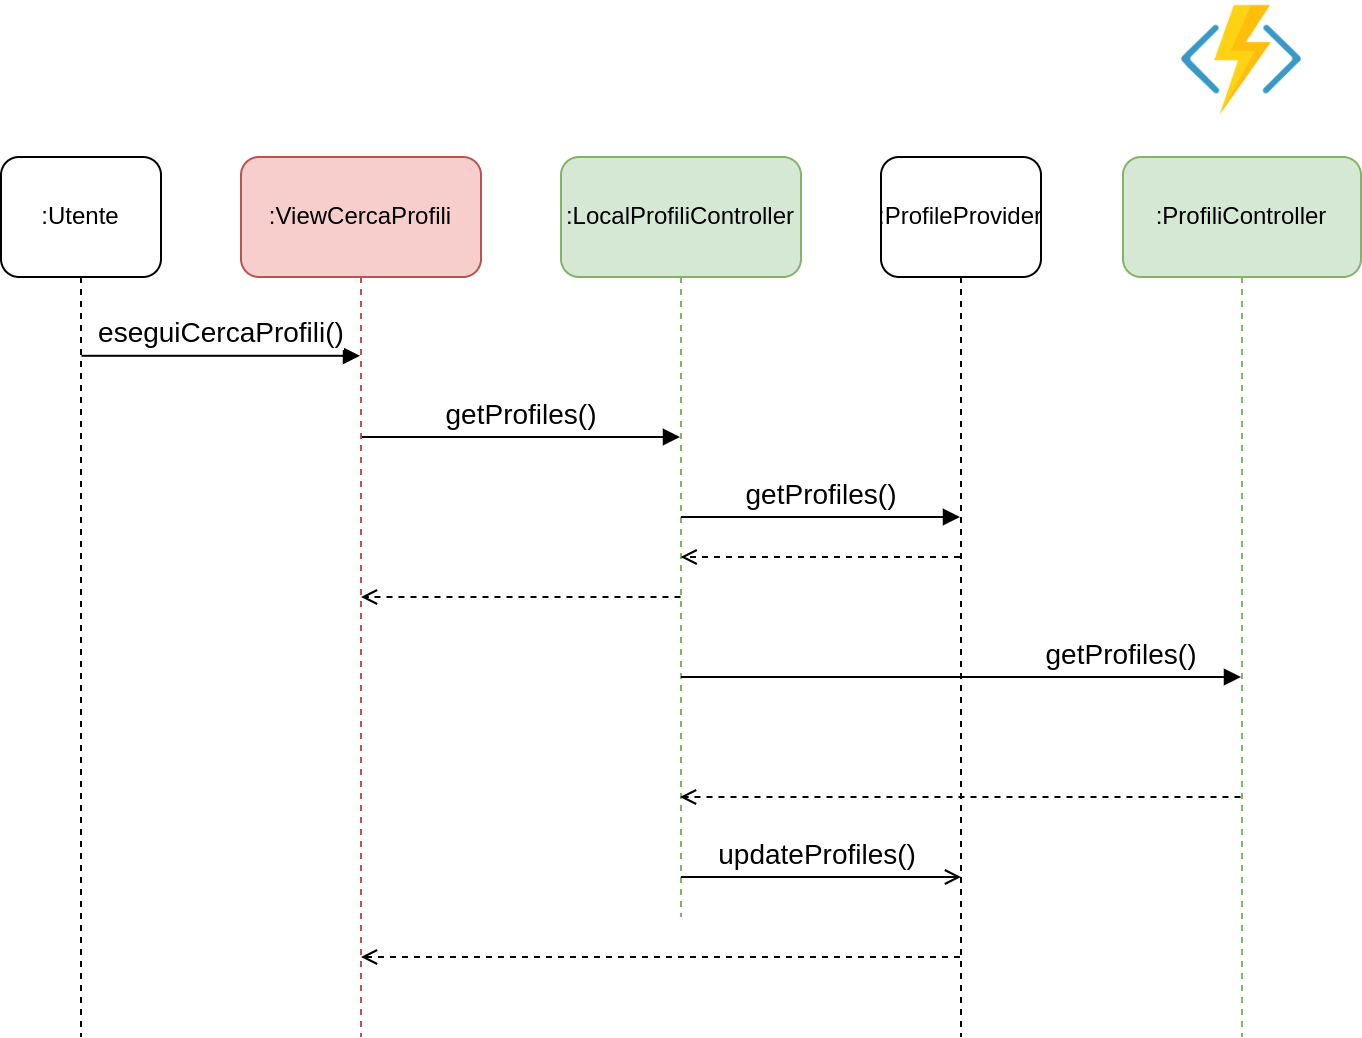
\includegraphics[width=\textwidth]{Providers.png}
    \caption{Esempio di interazione logica tra i componenti del client}
\end{figure}	

eventualmente salvataggio delle modifiche offline per caricarle quando si torna online. \\
\clearpage
\subsubsection{L'allineamento con la memoria centrale}

il client ha la responsabilità di tenere allineata la propria cache ai valori della memoria centrale. 
Per quanto possa fare temporaneamente affidamento sulle risorse che ha salvato in cache per ridurre i tempi di risposta con l’utente, 
la loro validità dipende dalla certezza che corrispondano ai dati ufficiali. \\
\\

Ogni elemento avrà associato l’ultimo momento in cui è stato aggiornato. 
Allo stesso modo, viene salvato l’ultimo momento in cui è stata attivamente effettuata una richiesta esplicita di aggiornamento.  
Ad ogni avvio dell’applicazione il client invierà una richiesta al server per ricevere tutti gli elementi che hanno subito modifiche successivamente al momento dell’ultimo aggiornamento.\\
\\
La necessità di avere aggiornati tutti gli elementi della cache nel minor tempo possibile dipende anche dalla tipologia dell’elemento. 
Bisogna identificare gli elementi per il quale l’allineamento è critico per il corretto funzionamento dell’applicazione, 
come invece quelli che svolgono ruoli secondari e possono essere aggiornati anche in un secondo momento. 
Ad esempio, la modifica della durata di un evento è necessario venga rilevata il prima possibile, 
mentre la modifica della foto associata ad un profilo ha vincoli di aggiornamento in memoria locale molto più rilassati.\\
\\
Nel caso di dati critici si implementa un meccanismo che esegue, periodicamente, una richiesta degli elementi modificati nell’arco di tempo dall’ultimo aggiornamento, 
per poi aggiornare il loro valore. Invece, nel caso di elementi secondari, 
si possono richiedere allineamenti direttamente nel momento in cui vengono posti espressamente in attenzione dato l’utilizzo dell’app.

\clearpage
\subsection{Aggiornamenti}

Data la natura condivisa dell’applicazione risulta fondamentale che gli utenti siano aggiornati in tempo reale sulle modifiche applicate agli eventi, 
oltre ad essere una prerogativa di tutte le applicazioni moderne, anche per migliorare la user experience. 
Lo spostamento di un appuntamento, la conferma di una presenza o la modifica del luogo di appuntamento sono elementi critici che è bene che gli utenti vengano informati il prima possibile. \\
\\
Il cloud fornisce strumenti per il supporto e lo sviluppo di queste funzionalità, ma, oltre a dover individuare la tecnologia più adatta, bisogna anche essere in grado di integrarla nel resto del progetto.\\
\\
\subsubsection{Scelta della tecnologia}


La comunicazione con il server finora implementata si basa sul protocollo Hypertext Transfer Protocol (HTTP). HTTP prevede un fornitore di servizi (il server) mettere a disposizione una porta ad un indirizzo fisso rimanendo in attesa di eventuali utilizzatori (client) che, interfacciandosi attivamente alla porta disponibile,  espongono le loro richieste.
La riduzione delle comunicazioni al minimo indispensabile, oltre a non richiedere al server alcuna conoscenza del client, rende il protocollo pratico e scalabile.

Questa dinamica però impedisce ai client di essere notificati di eventuali modifiche apportate, a meno di richieste periodiche frequenti che comportano un sovraccarico da entrambe le parti. Inoltre, l’inversione dei ruoli non è applicabile in quanto i client cambiano costantemente l’indirizzo a loro associato, così come è impossibile distinguere se il dispositivo abbia terminato la connessione o se sia un guasto di altro tipo. 

Si necessita una comunicazione che mantenga in costante contatto i client con le modifiche del server, permettendo una trasmissione attiva degli aggiornamenti.
A basso livello, il protocollo che permette una comunicazione continua più adatto alle tecnologie comunemente diffuse è quello delle WebSocket. Tramite WebSocket infatti si crea un canale diretto tra le parti che consente una comunicazione istantanea. 

Alla necessità di supportare il protocollo delle WebSocket e di inviare istantaneamente i messaggi, si aggiunge la possibilità di creare molteplici canali specifici per indirizzare correttamente le comunicazioni ai soli interessati.


\begin{figure}[h!]
    \centering
    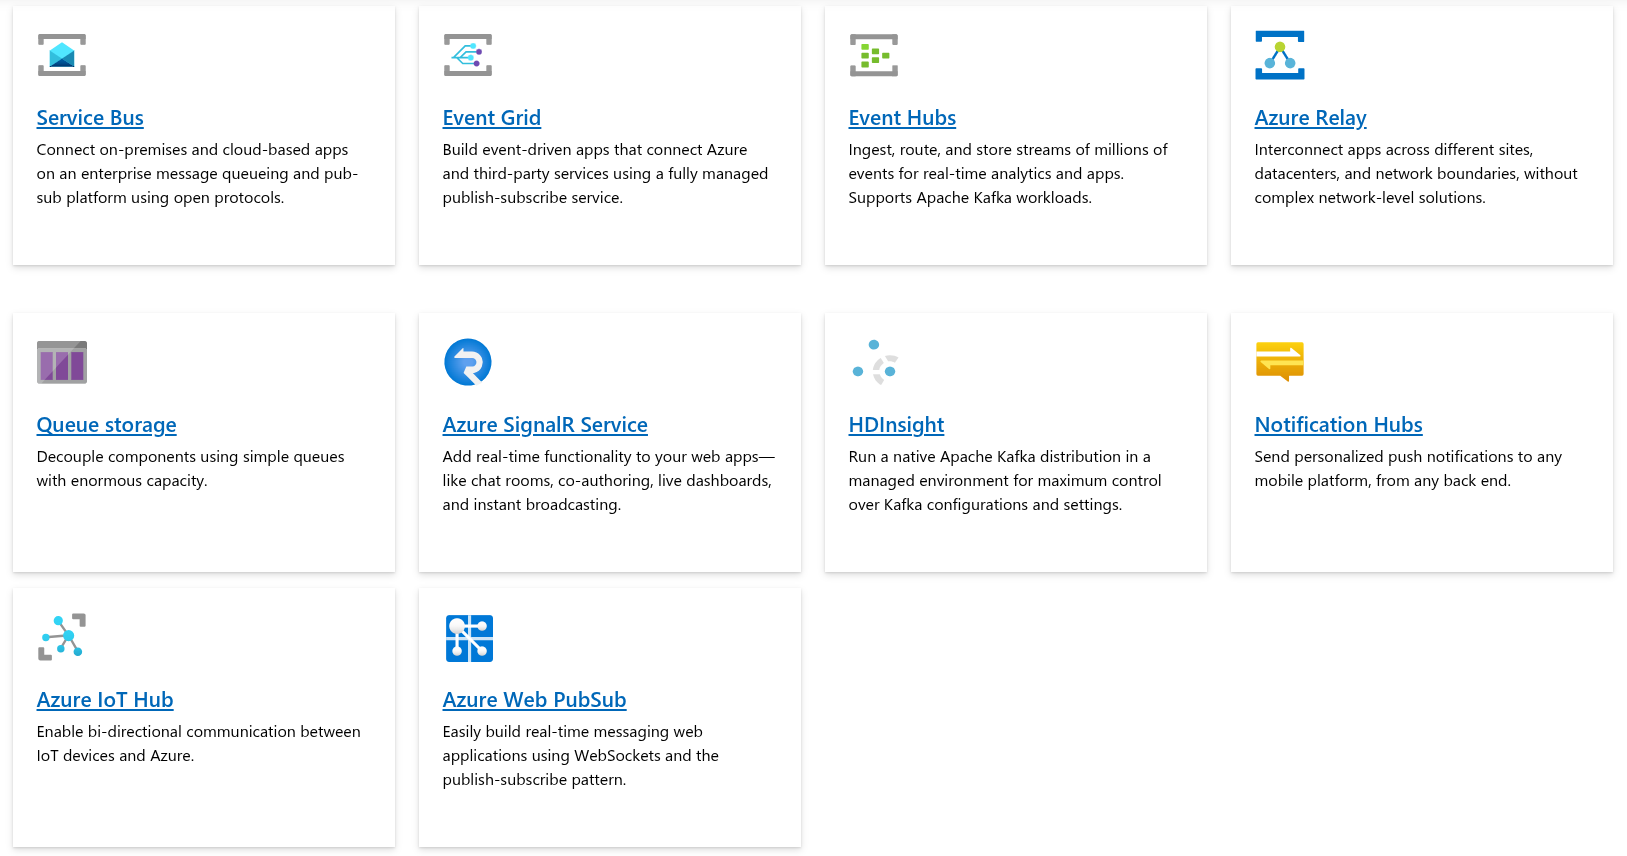
\includegraphics[width=\textwidth]{AzureMessagingServices.png}
    \caption{I servizi di comunicazione istantanea proprietari di Azure}
\end{figure}	


Per individuare la tecnologia più adatta ad aggiornare gli utenti, tra le tante che offrono servizi di collegamento istantaneo tra tecnologie, è fondamentale comprendere  gli scopi per cui sono nate e che problemi quindi risolvono. Infatti, ogni servizio è stato progettato per affrontare specifiche sfide che si differenziano sia per la natura dei servizi a cui si rivolgono che per  modalità di approccio .

La natura degli attori per cui il servizio si specializza determina le prestazioni di scalabilità e le integrazioni supportate. Bisogna quindi considerare la località e la natura delle risorse: in-premise o sul cloud, se appartengono alla stessa piattaforma o se devono comunicare internamente.
Ad esempio, un servizio pensato per collegare tantissimi dispositivi distribuiti con limitato potere computazionale, come nel caso dell’Internet of Things, fornirà  supporto a connessioni esterne e a protocolli standard, e prevederà un’elevata quantità di richieste di limitate dimensioni e frequenza. Viceversa, la necessità di creare una comunicazione tra un numero ristretto di server con prestazioni elevate comporta la creazione di flussi di dati importanti, magari gestiti internamente all’ambiente cloud, astraendo la tecnologia necessaria.

I servizi si differenziano però anche per le caratteristiche delle connessioni gestite.
Proprietà fondamentale è la natura delle comunicazioni. I canali possono essere infatti unidirezionali, permettere la comunicazione da entrambe le parti o implementati come flussi di eventi, in cui le comunicazioni possono essere inviate e ricevute da molteplici attori, senza che il destinatario sia noto al mittente. Inoltre, alcuni servizi offrono la possibilità di individuare categorie di clienti specifiche a cui eventualmente inviare notifiche mirate. Infine, bisogna prendere in considerazione la necessità di persistenza delle comunicazioni, che fornisce, oltre all’aggiornamento in tempo reale, anche la possibilità di recuperare modifiche passate.

Nel progetto si necessita di un servizio che supporti le WebSocket e che permetta di creare una molteplicità di canali unidirezionali differenti. In particolare, deve essere il più indipendente possibile dagli attori con cui comunica per poter garantire il maggior supporto possibile. Dovendo coprire solo le notifiche di aggiornamento, senza responsabilità di rintracciabilità dei dati, la presenza della persistenza non è necessaria.

Gratuito per le prime 20 connessioni, ma eventualmente scalabile per soddisfare ulteriori carichi, il servizio individuato per la gestione delle notifiche in tempo reale è Azure Web Pub Sub (AWPS). Permette infatti la creazione di canali tramite WebSockets e l’integrazione con le Azure Functions. Supporta la creazione di canali, sia unidirezionali che bidirezionali, su cui pubblicare eventi, a cui gli utenti possono collegarsi per ricevere gli aggiornamenti. Non prevede l’utilizzo di persistenza ma gestisce completamente la scalabilità e l’affidabilità del sistema.



\subsubsection{Integrazione}

L’integrazione di Azure Web Pub Sub deve avvenire sia con il server che con i devices degli utenti. Seguendo il modello publish subscribe, ogni client si connetterà ad un canale in sola lettura, ricevendo tutti i dati che verranno pubblicati su di esso. Il server avrà il compito di interfacciarsi con il servizio per pubblicare i dati sui canali interessati.

La scelta della definizione del canale deriva da un’ulteriore analisi del dominio. 
Il soggetto interessato alle modifiche sottoposte a notifica è il profilo. 
Se però si creassero i canali in relazione ai profili ogni dispositivo (che riassume l’interazione di un utente) dovrebbe mantenere una connessione per ogni profilo collegato all’utente. La creazione di un canale per ogni device allo stesso modo risulta estremamente inefficiente, in quanto, oltre ad introdurre nuovi requisiti per garantire la tracciabilità dei dispositivi, ne richiederebbe di creazione e gestione in numero elevato. Per queste ragioni i canali verranno creati uno per utente, garantendo inoltre che gli unici utenti a ricevere le notifiche ne posseggano effettivamente l’accesso adeguato.

A seguito di una richiesta che comporta la notifica ai profili interessati, il server avrà il compito di interfacciarsi con AWPS per affidargli le comunicazioni relative. Tuttavia AWPS non supporta la capacità di unire gli elementi in base alle loro relazioni, per cui la responsabilità di trovare gli utenti interessati ricade sul server. 
Ad esempio, la modifica di un evento comporta la notifica a tutti i profili relativi, e quindi una comunicazione a tutti gli utenti che ne posseggono i permessi di notifica per la particolare azione su detti profili. 

L’operazione di ottenimento degli utenti coinvolti data l’azione svolta (nell’esempio, la modifica di un evento) verrà eseguita in un’altra Azure Functions dedicata che si occuperà poi, per ogni utente coinvolto, di comunicare  al server AWPS il messaggio da notificare. L’eventuale fallimento della operazione viene inserito tra i log e risulterà durante i monitoraggi, senza coinvolgere la funzione principale.

		
\begin{figure}[h!]
    \centering
    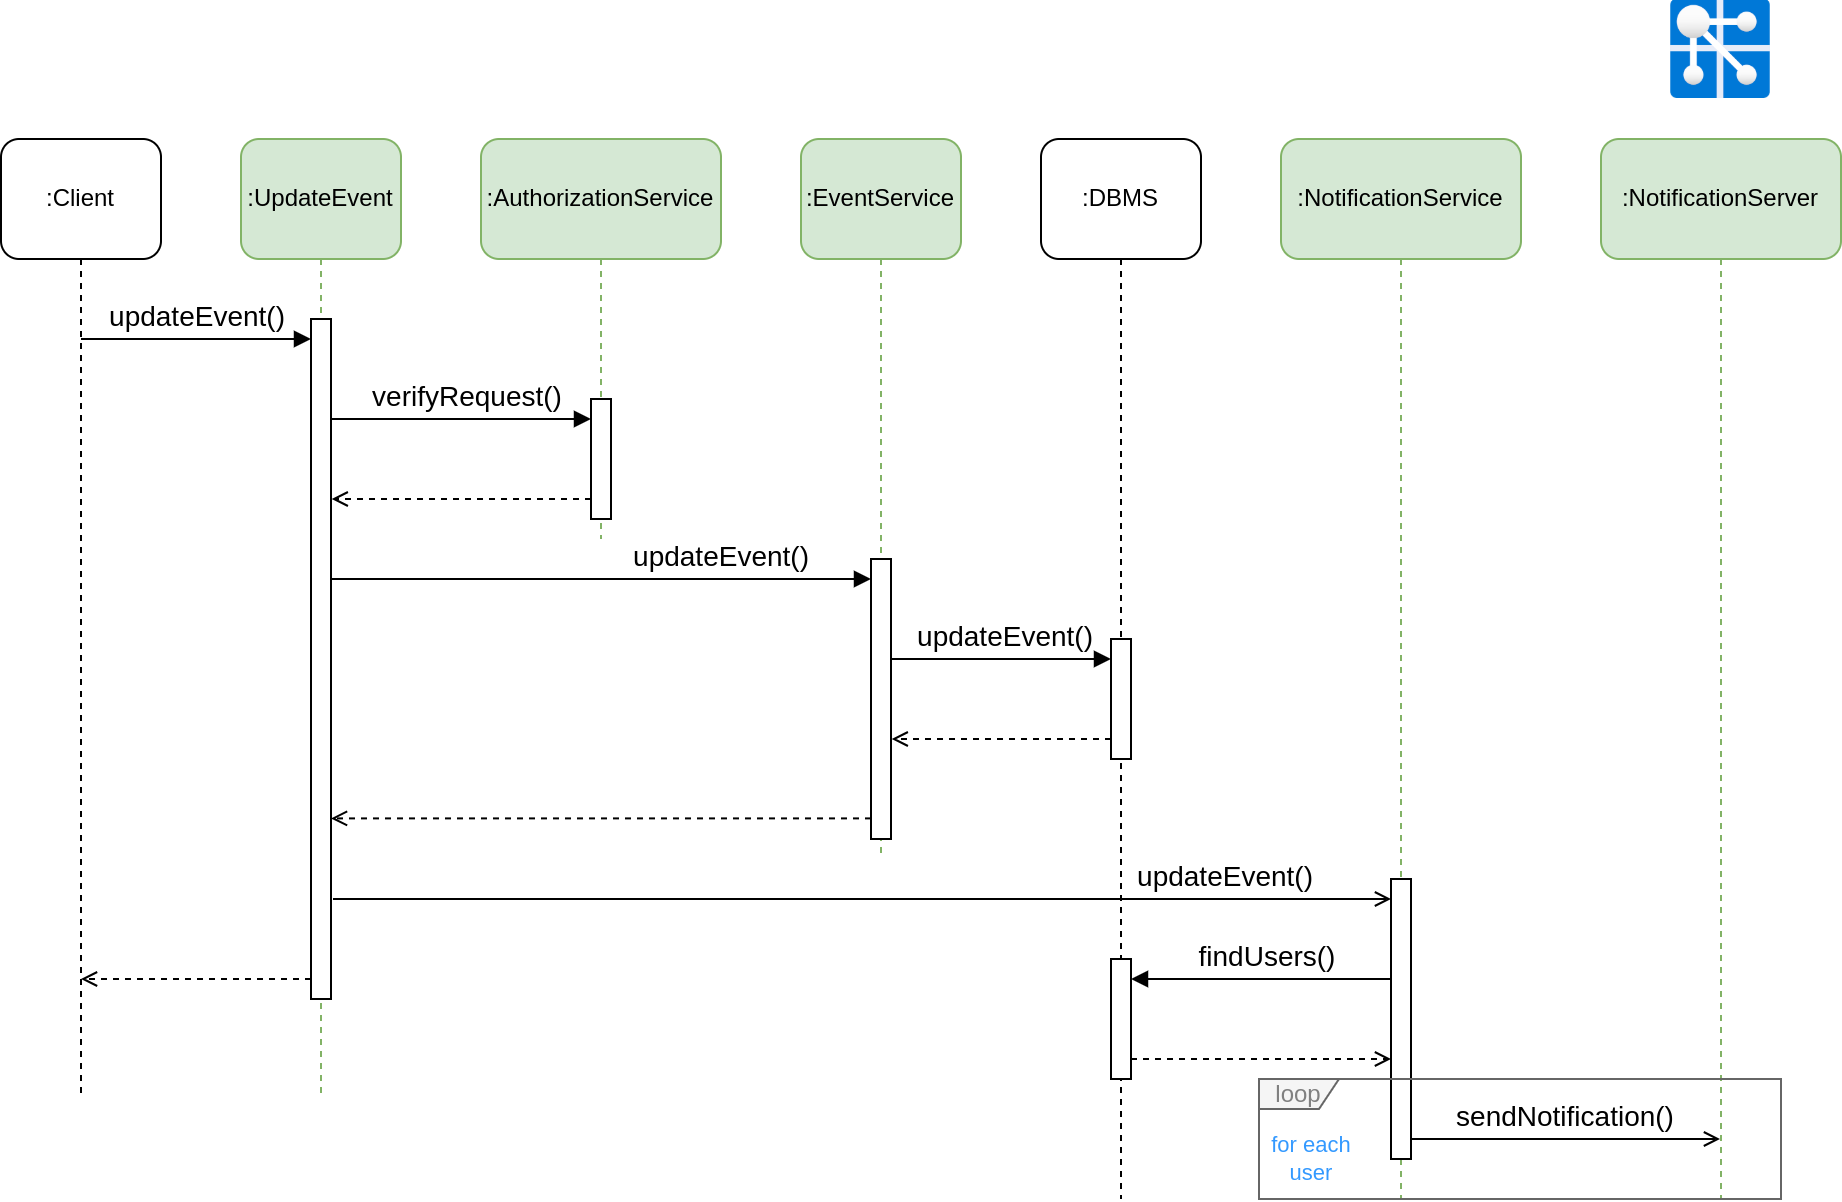
\includegraphics[width=\textwidth]{IIModificaEvento2.png}
    \caption{Interazione delle Azure Functions con AWPS}
\end{figure}	

La ricezione della notifica sul dispositivo dell’utente può comportare la richiesta al server dell’elemento modificato. La scelta di recuperare i dati tramite il server invece di includere i dati direttamente all’interno della notifica permette di uniformare il formato delle notifiche, semplificando la loro gestione e velocizzando l'invio; di diminuisce il volume dei dati trasmessi tramite WebSocket, garantendo la scalabilità delle notifiche; di migliorare la gestione degli errori da parte del server rendendoli più affidabili e di garantisce la possibilità di recuperare solo l’ultimo aggiornamento, riducendo il consumo totale dei dati.


\begin{figure}[h!]
    \centering
    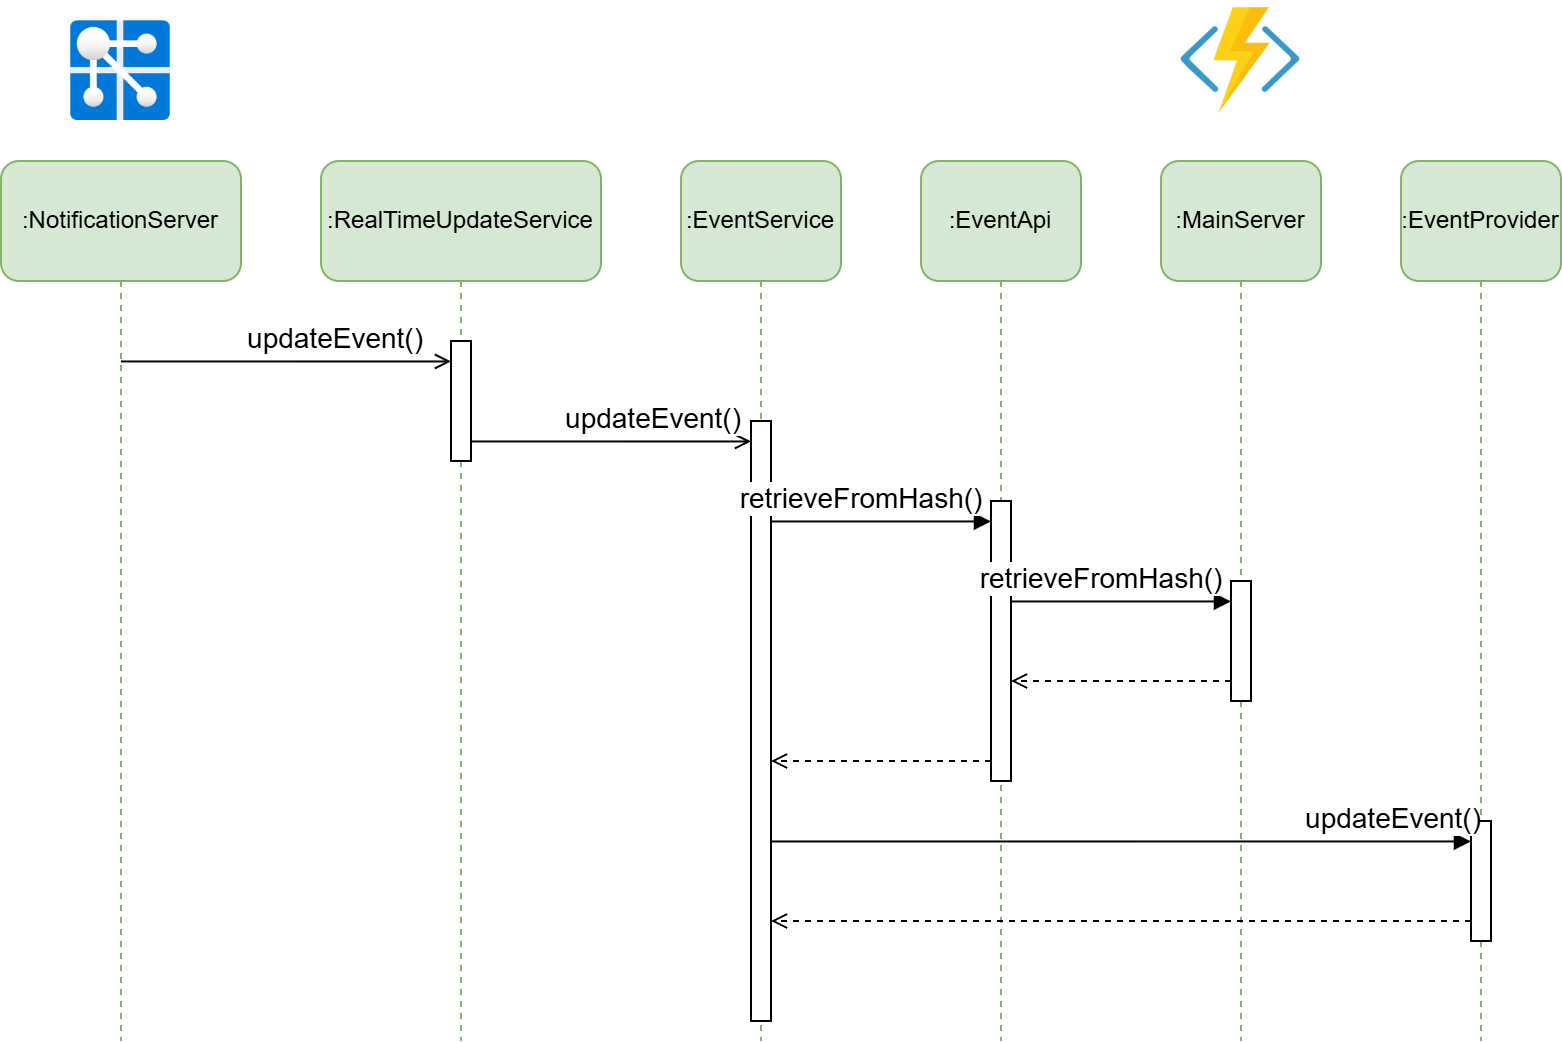
\includegraphics[width=\textwidth]{IIAggiornaEvento.png}
    \caption{Interazione tra AWPS e un client}
\end{figure}	

\clearpage